% This template was initially provided by Dulip Withanage.
% Modifications for the database systems research group
% were made by Conny Junghans,  Jannik Strötgen and Michael Gertz

\documentclass[
     12pt,         % font size
     a4paper,      % paper format
     BCOR10mm,     % binding correction
     DIV14,        % stripe size for margin calculation
     ]{article}

%%%%%%%%%%%%%%%%%%%%%%%%%%%%%%%%%%%%%%%%%%%%%%%%%%%%%%%%%%%%

% PACKAGES:

% Use German :
\usepackage[english]{babel}
% Input and font encoding
\usepackage[latin1]{inputenc}
\usepackage[T1]{fontenc}
\usepackage[title]{appendix}
% Index-generation
\usepackage{makeidx}
% Einbinden von URLs:
\usepackage{url}
\def\UrlBreaks{\do\/\do-}
% Special \LaTex symbols (e.g. \BibTeX):
%\usepackage{doc}
% Include Graphic-files:
\usepackage{graphicx}
% Include doc++ generated tex-files:
%\usepackage{docxx}

% Fuer anderthalbzeiligen Textsatz
\usepackage{setspace}

\usepackage{amsmath}
\usepackage{amssymb}
% F�r todos
\usepackage[obeyFinal]{easy-todo}

% hyperrefs in the documents
\PassOptionsToPackage{hyphens}{url}\usepackage[
  bookmarks=true,
  colorlinks,
  pdfpagelabels,
  pdfstartview = FitH,
  bookmarksopen = true,
  bookmarksnumbered = true,
  linkcolor = black,
  plainpages = false,
  hypertexnames = false,
  citecolor = black,
  urlcolor=black]{hyperref}
%\usepackage{hyperref}

% subfigures
\usepackage{subcaption}


%%%%%%%%%%%%%%%%%%%%%%%%%%%%%%%%%%%%%%%%%%%%%%%%%%%%%%%%%%%%

% OTHER SETTINGS:

% Choose language
\newcommand{\setlang}[1]{\selectlanguage{#1}\nonfrenchspacing}

% Written by comment
\newcommand{\comment}[1]{\vspace{-1em}\hspace{27pt}{\small\textit{#1}}\bigskip\par}
\newcommand{\subcomment}[1]{\vspace{-0.8em}\hspace{35pt}{\small\textit{#1}}\bigskip\par}
\newcommand{\subsubcomment}[1]{\vspace{-0.8em}\hspace{39pt}{\small\textit{#1}}\bigskip\par}

\setcounter{tocdepth}{2} 

\begin{document}

% TITLE:
\pagenumbering{roman} 
\begin{titlepage}


\begin{center}
\textbf{ 
\Large Heidelberg University\\
\smallskip
\Large Institute of Computer Science\\
\smallskip
\Large Database Systems Research Group\\
\smallskip
}

\vspace{2cm}

\textbf{\large Project Report - Text Analytics}

\vspace{0.5\baselineskip}
{\huge
\textbf{Scientific Papers Clustering}
}
\end{center}

\vfill 

{\large
\begin{tabular}[l]{ll}
Team Member: & Daniela Fichiu, 3552717,\\& BSc Applied Computer Science,\\
  & BSc Mathematics\\
  & daniela.fichiu@stud.uni-heidelberg.de\\
Team Member: & Christian Homeyer, 3606476,\\ & PhD Computer Science \\
  & ox182@uni-heidelberg.de\\
Team Member: & Jessica Kaechele, 3588787,\\ & MSc Applied Computer Science\\
  & Uo251@stud.uni-heidelberg.de\\
Team Member: & Jonas Reinwald, 3600238, \\ & MSc Applied Computer Science\\
  & am248@stud.uni-Heidelberg.de\\
Mentor: & Dennis Aumiller
  
\end{tabular}
}
\vspace*{1cm}

{
  \textbf{GitHub Repository: \url{https://github.com/DonatJR/ita_ws20}}
}
\vspace*{.5cm}

\begin{center}
{
We  hereby  declare  that  all  material  in  this  project  is  our  own  work except where there is clear acknowledgement or reference to the work of others. } 
\end{center}


\end{titlepage}

\pagenumbering{arabic} 

% \input{<file>}
\newpage
\tableofcontents

\listoffigures
\listoftables

\newpage
\section{Abstract}
\subsection{Introduction}

\subcomment{Written by Daniela Fichiu}
If you type a query like "how do I open the terminal on mac?" into Google, you already know what you want to find: a set of steps that will open a terminal on the screen.

Most would say doing homework is, on the best days, an unpleasant affair. But everyone would agree that writing an assignment for that one course you've always skipped is a chore. You most certainly do not understand the airy slides. Your only option is to search for materials on your own - extensive research is needed to find the materials that can fill all your knowledge gaps.

A student who wants to know more about text analytics might search for "text analytics" on Google Scholar. The query yields back 1.650.000 results, the top three being "Text Analytics with Python," "Text analytics in social media," and "Semantic interaction for visual text analytics." A subsequent query like "text analytics topics" yields back results with the following titles: "Analyzing educational comments for topics and sentiments: A text analytics approach" or "A text analytics approach for online retailing service improvement: Evidence from Twitter."

We know how time-consuming it is to spend hours on search engines or websites like Research Gate or Google Scholar looking for research papers, hoping for the best, but never quite finding the perfect materials.

Our project emerged from the need to find an easy way of exhaustively searching for scholarly literature while bringing to light the relations between the subfields of the research field of interest and other areas. Our goal is to provide a deeper understanding of the material to be searched for and easing up the process of finding information.

We propose a solution that clusters scientific texts into relevant subgroups. The subgroups can then be more easily presented to and explored by people looking for specific topics and terms.

We focus on a subset of around two thousand papers from the field of machine learning. We cluster the research papers, extract a ground truth using the papers' keywords, and compare the clustering results against the ground truth. We also prove that an unbalanced data set can have a significant impact on the clustering results. 

Even with the conclusions written down, we do not see our work as finished. The proposed pipeline could be usable on a broader range of fields. We also intend to balance our data set by adding research papers from other areas.

We also believe that our solution, supported by good group visualization tools and a user-friendly search interface, can be successfully integrated into a metasearch site.
\section{Related Work}
\comment{Written by Jessica Kaechele}

There exist various approaches to simplify getting an overview of a research field without extensive research and reading countless papers. By browsing through digital libraries and search engines you can find papers by matching search strings, but to get an overview of an entire research field this is not enough.
In \cite{Rapid_understanding_of_scientific_paper_collections} a tool is presented that uses different methods to gain insights into research fields.
Through the citation network, papers can be divided into clusters.
Another possibility to get insights is the citation context because the key statements of the paper are often summarized concisely.  To know the key statements of the paper, it is still necessary to read the whole paper or at least all citation contexts. For many papers, this is still a very large amount of work. To solve this problem Multi-Document Summarization is used. This summarization is only applied to abstract and citation context.

With the help of the techniques mentioned, it should be possible to gain insight into an entire research field more quickly.
In this project, the focus is only on clustering.
For many years, attempts have been made to cluster papers in order to simplify the research. In 1973, for example, it had already been tried to cluster journals by comparing reference patterns and looking at mutual references \cite{Clustering_of_scientific_journals}.

In \cite{Document_clustering_of_scientific_texts_using_citation_contexts} the context of the citations is used in addition to the citations to cluster.
First, a citation has to be recognized and the text has to be extracted on both sides of the citation. Then different clustering approaches are applied and compared. In addition, this technique is also applied to the entire document and compared to the approach of citation context.

In this project, we do also want to use different clustering approaches.
But when examining the citation contexts, access to the entire paper is required. Besides, it is difficult to identify citations in PDFs because of the different ways of citing. Abstracts, on the other hand, are commonly available and no further extraction step is needed.

There are already some approaches that are using abstracts for clustering.
In \cite{Clustering_scientific_documents_with_topic_modeling} abstracts and titles are used.

Two types of pre-processing are performed on the texts. 
%The first method treats each word as a token, and stopwords are deleted. The second method uses term-clumping to find noun phrases with significant commonality.
Afterward, several topic modeling algorithms are used. 
The clusters created by the algorithms have to be named manually.

In our project, a similar preprocessing is done.
Additionally to some topic modeling approaches different clustering algorithms are tested to find out which algorithm fits best to our dataset. 
Furthermore, a dimensionality reduction will be tested to improve the clustering and the clusters will be named automatically in this project.

Abstracts are also used in \cite{An_Approach_to_Clustering_Abstracts} to perform clustering, by preprocessing, calculating the cosine similarity, and using different clustering methods.
%First tokenization is used, then stopwords are removed and a stemming algorithm is performed.
%Because of the shortness of abstracts, the words must have a higher frequency than in a generally balanced corpus of the given language. Then the keywords are grouped and weighted and the closeness of the two documents is calculated using cosine similarity measure. 
%Additionally, clustering methods are applied to the whole abstract. Three algorithms from three different approaches are used: the k-medoid method from the example-based approach, the nearest neighbor method from the hierarchy-based approach, and the MajorClust method from the density-based approach.
As dataset 48 abstracts are used, which have been classified by a human.

Again, a similar approach to ours is used. However, with only 48 abstracts, there is a high risk of over-fitting and bias.
This is to be avoided in this project.
\section{Method}

\subsection{Clustering}
There are plenty of different clustering algorithms, that perform differently depending on the nature of the data.
The algorithms tested in this project are described below.

\subsubsection{K-Means}
\subsubcomment{Written by Jessica Kaechele}
The goal of K-Means is that data points that are within a cluster are as similar as possible, while two different clusters are as different as possible.
To achieve this, a centroid is randomly selected for each of the $k$ clusters.
Then the sum of squared distance between each data point and the cluster centroid are calculated.
Based on this calculation, the data points are assigned to the closest centroid.
Now, new centroids per cluster are calculated by taking the average of all data points within that cluster.
These steps are repeated until the centroids no longer change.\cite{kmeans}

With K-Means, the number of clusters $k$ must be defined. If $k$ is not known, it can be determined using the elbow method, for example.
In this method, the sum of squared distances between the data points and their cluster centroid is calculated for different $k$.
It can often be seen that the sum of squared distances drops significantly at the beginning and then remains at approximately the same level.
The optimal $k$ can be found at the point where the curve starts to flatten out.\cite{kmeans}

\subsubsection{Spectral Clustering}
\subsubcomment{Written by Jessica Kaechele}
Spectral Clustering already includes a dimensionality reduction.
The first step is to construct a similarity graph.
Each vertice $v_i$ represents a data point $x_i$.
An edge between two vertices $v_i$ and $v_j$ exists if the similarity $s_ij$ is higher than a previously defined threshold.
These similarities can be used as weights $w_ij$ in a weight matrix $W$.
If there is no edge between two vertices, the weight is $0$.
With the help of this weight matrix, a degree matrix can be calculated.
Therefore, the degree is calculated for each vertice by summing the weights:
$$
d_i = \sum_{j=1}^n{w_{ij}}
$$
Then the graph laplacian matrix is calculated by subtracting the weight matrix from the degree matrix:
$$
L = D - W
$$
Afterwards, the first $k$ smallest eigenvectors of the matrix $L$ are calculated.
Finally, the newly created data points are clustered using K-Means.\cite{spectral_clustering}

The graph laplacian matrix can also be calculated as a normalized graph laplacian \cite{spectral_clustering}.
This changes the algorithm slightly, but this is not discussed in detail here, as the functionality of the algorithm does not change.

\subsubsection{BIRCH}
\subsubcomment{Written by Jessica Kaechele}
BIRCH also reduces the scale of the dataset by defining subclusters.
These subclusters are called clustering features(CF).
The information that is retained is the number of data points that are included, the linear sum of the included data points, and the squared sum.
Also, a CF can contain other CFs.
The CFs are now arranged in a tree, with each node containing at most $B$ entries.
An entry in a non-leaf node consists of a CF and a pointer to a child node.
A leaf node consists of at most $L$ CFs.
In addition, there is a threshold $T$, which determines the maximum diameter of the entries of the leaf node.
The diameter is the average pairwise distance within a cluster.

If a new CF or data point is inserted, the tree is descended recursively by selecting the closest child node based on a distance metric.
Once a leaf node is reached, the closest CF entry is searched for, which can absorb the new CF entry without exceeding $T$.
However, if $T$ is exceeded, a new CF entry is appended.
If the leaf node already contains $L$ entries, it must be split.

Now all CF entries of the parent nodes are updated.
In case of a split, a new entry must be added to the parent node.
If $B$ entries are already contained there, this node must also be split again, etc.

When building the tree it is ensured that the complete tree can be loaded in the memory by increasing $T$ if necessary.
The clustering is performed by any clustering algorithm, which clusters the CFs in the leaf nodes.\cite{birch}
%\subsection{Dimensionality Reduction}
It is possible to perform a dimensionality reduction before doing the clustering.
This often reduces the computation time, and by using only the most important features of the data, the results can sometimes be improved.  

\subsubsection{Latent Semantic Analysis }
\subsubcomment{Written by Jessica Kaechele}
In addition to Topic Modelling, Latent Semantic Analysis (LSA) can also be used for the dimensionality reduction of texts.
The documents are first represented as a term-document matrix, where the rows represent a word and the columns represent a document.
The cells contain the frequency in which the terms occur in a document.
The TF-IDF matrix is then calculated from this matrix, by multiplying frequencies with the inverse document frequency.
Afterward, a singular vector decomposition is performed.\cite{lsa}

\subsubsection{Spectral Embedding}\label{subsubsec:spectral_embedding}
\subsubcomment{Written by Jonas Reinwald}
Spectral Embedding is a general approach for calculating non-linear embeddings. It has locality preserving properties\cite{spectral_embedding_paper}, making it useful for clustering low-dimensional representations of higher dimensional data.
It works by first constructing an adjacency graph where nodes are connected if they are close to each other. If they are close can be determined by a number of ways, in our experiments we only use a nearest neighbor approach. The edges between close nodes are then weighted and a graph Laplacian is constructed from it. Next, eigenvalues and eigenvectors of the graph Laplacian are computed. Skipping the first eigenvector, the next m eigenvectors are used for embedding in m-dimensional space.\cite{spectral_embedding_paper}


\section{Experimental Setup and Results}

\subsection{Results and Analysis}

In the following sections, results from each method discussed in chapter \ref{clustering_methods} are shown and described.
The scores used in this chapter are from our notebook experiments as we worked with them for the majority of the project duration and are thus most familiar with them. Results from the main clustering pipeline with similar parameters can and will differ slightly.

\subsubsection{LDA and LSA}
\subsubcomment{Written by Jessica Kaechele}
By using the topic modelling methods LSA and LDA, first insights into the nature of the data can be gained.

Table \ref{tab:lda_lsa_topwords} shows the top words of each cluster when forming two clusters using LDA and LSA.
\begin{table}[]
    \centering
    \caption{Top words of two clusters retrieved by LDA and LSA}
    \begin{tabular}{l|l|l|l}
        \multicolumn{2}{c}{LDA} & \multicolumn{2}{c}{LSA} \\
        Cluster 1 & Cluster 2 & Cluster 1 & Cluster 2\\
        \hline
        \shortstack[l]{alexey \\ bibliography \\ chervonenkis \\ preface \\ synergy \\ comment \\ deap \\ repeating \\ manopt \\ introductory} & \shortstack[l]{model \\ learning \\ algorithm \\ data \\ method \\ problem \\ function \\ matrix \\ kernel \\ regression} & \shortstack[l]{model \\ graph \\ network \\ graphical \\ inference \\ latent \\ causal \\ data \\ variable \\ gaussian} & \shortstack[l]{model \\ algorithm \\ learning \\ data \\ method \\ problem \\ function \\ matrix \\ kernel \\ regression} 
    \end{tabular}
    \label{tab:lda_lsa_topwords}
\end{table}
While the terms describing cluster 2 are very general, those of cluster 1 are very specific.
In the case of LDA, they even include names.
This indicates that many papers are assigned to cluster 2 and only a few to cluster 1.
This can also be observed when extracting more than two clusters.
The visualization in 2 dimensions, which can be seen in figure \ref{fig:lda_lsa}, strengthens this assumption.
\begin{figure}
\centering
\begin{subfigure}{.4\textwidth}
  \centering
  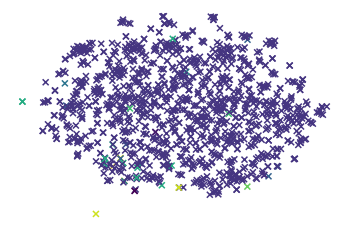
\includegraphics[width=\linewidth]{imgs/lda.png}
  \caption{LDA}
  \label{fig:lda}
\end{subfigure}%
\begin{subfigure}{.4\textwidth}
  \centering
  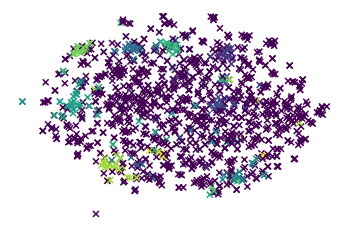
\includegraphics[width=\linewidth]{imgs/lsa.png}
  \caption{LSA}
  \label{fig:lsa}
\end{subfigure}
\caption{two-dimensional representation of 15 clusters}
\label{fig:lda_lsa}
\end{figure}
In the case of LDA, a large proportion of the papers are assigned to one cluster, while other clusters appear only rarely.
With LSA, a few small clusters can be identified, but these are located within a large cluster.

These results are also found in the evaluation metrics, as can be seen in table \ref{tab:scores_lsa_lda}.
\begin{table}[]
    \centering
    \begin{tabular}{c|c|c|c}
     Model & Silhouette Score & Calinski-Harabasz-Score & Davies-Bouldin-Score  \\
     \hline
     \hline
     LDA & -0.0026 & 1.1233 & 2.6217 \\
     \hline
     LSA & -0.0089 & 2.9692 & 4.4138
    \end{tabular}
    \caption{Metrics retrieved with LSA and LDA extracting 15 clusters}
    \label{tab:scores_lsa_lda}
\end{table}
The Calinski-Harabsz-Score is very low and the Silhouette Score is even negative.
The reason for this could be that the clusters are not clearly separated from each other.
The Davies-Bouldin-Score, however, seems to indicate better results, especially for LDA.
The reason for this could be that a cluster sometimes only consists of one paper and therefore the average distance between each point of the cluster and its cluster center is very low.

Both the metrics and the visual representation suggest that LSA and LDA are not suitable clustering algorithms for our data.


\subsubsection{K-Means}\label{subsubsec:kmeans}
\subsubcomment{Written by Jessica Kaechele}
Before clustering with K-Means, it is necessary to find a suitable number of clusters using the Elbow Method.
In figure \ref{fig:elbow} it can be seen that no kink is formed and therefore the number of clusters cannot be determined.
\begin{figure}
    \centering
    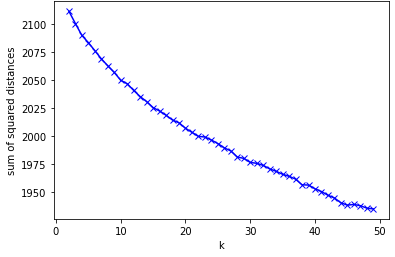
\includegraphics[width=0.5\linewidth]{imgs/elbow.png}
    \caption{Elbow Method with K-Means}
    \label{fig:elbow}
\end{figure}
The reason for this can be clearly seen in figure \ref{fig:kmeans_no_dim}. Because a cluster contains fewer data points the more clusters have formed the sum of squared distances becomes smaller.
But an ideal value for $k$ does not arise, because of the centroids which are all located exactly in the center of the dataset.

If a dimensionality reduction using LSA or Spectral Embedding is applied before clustering, an elbow can be seen.
The data is reduced to two components, with both dimensionality reduction methods, since it leads to the best scores.
Additionally, the optimal number of clusters seems to be 15 since the elbow flattens at this point.
The scores improve significantly compared to K-Means without dimensionality reduction as can be seen in table \ref{tab:scores_kmeans}. Visually, clusters are now clearly visible and the cluster centroids are better distributed.
This can be seen in figure \ref{fig:kmeans}.

\begin{figure}
\centering
\begin{subfigure}{.3\textwidth}
    \centering
    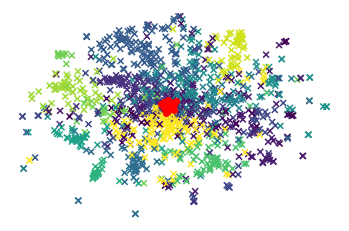
\includegraphics[width=\linewidth]{imgs/kmeans.png}
    \caption{No dimensionality reduction}
    \label{fig:kmeans_no_dim}
\end{subfigure}
\begin{subfigure}{.3\textwidth}
  \centering
  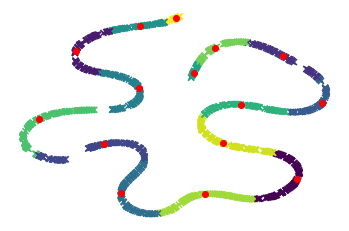
\includegraphics[width=\linewidth]{imgs/kmeans_lsa.png}
  \caption{LSA}
  \label{fig:kmeans_lsa}
\end{subfigure}%
\begin{subfigure}{.3\textwidth}
  \centering
  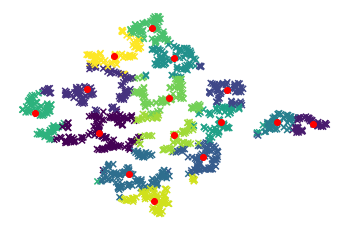
\includegraphics[width=\linewidth]{imgs/kmeans_spectral.png}
  \caption{Spectral Embedding}
  \label{fig:kmeans_spectral}
\end{subfigure}
\caption{two-dimensional representation of 15 clusters retrieved by K-Means with their centroids with different dimensionality reductions}
\label{fig:kmeans}
\end{figure}


\begin{table}[]
    \centering
    \begin{tabular}{c|c|c|c}
     Model &  \shortstack[c]{Silhouette \\ Score} & \shortstack[c]{Calinski-Harabasz \\ Score} &  \shortstack[c]{Davies-Bouldin \\ Score}  \\
     \hline
     \hline
     K-Means & 0.0103 & 7.303 & 7.7293 \\
     \hline
     \shortstack[c]{K-Means with \\ LSA} & 0.521 & 16793.344 & 0.53472 \\
     \hline
     \shortstack[c]{K-Means with \\ Spectral Embedding} & 0.3402 & 1813.0376 & 0.834 \\
     \hline
     \shortstack[c]{K-Means \\ with LSA and \\ custom stopword removal} & 0.5336 & 14589.2349 & 0.5109 \\

    \end{tabular}
    \caption{Metrics retrieved with K-Means extracting 15 clusters}
    \label{tab:scores_kmeans}
\end{table}


It can be observed that terms like \textit{algorithm}, \textit{method}, \textit{data} appear in the top words of many clusters.
By removing these words, it might be possible to separate the clusters even better. 
But it turns out, that although these terms no longer appear, other terms do show up, which appear in many clusters.
Besides, the metrics in table \ref{tab:scores_kmeans} show that the clusters hardly change.
Only the Calinski-Harabasz-Score deteriorates significantly. This indicates that the clusters are now no longer as dense or easily separable.


\subsubsection{Spectral Clustering}
\subsubcomment{Written by Jessica Kaechele}
Since Spectral Clustering consists of Spectral Embedding and K-Means, it should yield similar results to those obtained in section \ref{subsubsec:kmeans}.
However, this is not the case.
The Silhouette Score is only $0.0117$, the Calinski-Harabasz-Score is $4.57$ and the Davies-Bouldin-Score is $6.518$.
If one compares these values with the results obtained using Spectral Embedding and K-Means (see table \ref{tab:scores_kmeans}), it can be seen that the results are significantly worse.
The reason for this could be different parameters.
However, even after using the same parameters in both approaches, it is not possible to achieve similarly good results. 
Why the results are so different needs further investigation.



\subsubsection{BIRCH}
\subsubcomment{Written by Jessica Kaechele}
Similar to K-Means, BIRCH combined with a dimensionality reduction achieves better results, as can be seen in table \ref{tab:scores_birch}.
\begin{table}[]
    \centering
    \begin{tabular}{c|c|c|c}
     Model &  \shortstack[c]{Silhouette \\ Score} & \shortstack[c]{Calinski-Harabasz \\ Score} &  \shortstack[c]{Davies-Bouldin \\ Score}  \\
     \hline
     \hline
     BIRCH & 0.0017 & 4.056 & 6.8339 \\
     \hline
     \shortstack[c]{BIRCH with \\ LSA} & 0.4852 & 6294.5856 & 0.4793
 \\
     \hline
     \shortstack[c]{BIRCH with \\ Spectral Embedding} & 0.3238 & 1007.1024 & 0.8867 \\
     \hline
     \shortstack[c]{BIRCH \\ with LSA and \\ custom stopword removal} & 0.4984 & 7511.1226 & 0.8867 \\

    \end{tabular}
    \caption{Metrics retrieved with BIRCH extracting 15 clusters}
    \label{tab:scores_birch}
\end{table}
This can also be seen in the two-dimensional representation(see figure \ref{fig:birch}) where the clusters look well separated with LSA and Spectral Embedding.
\begin{figure}
\centering
\begin{subfigure}{.3\textwidth}
    \centering
    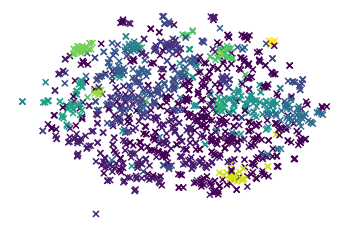
\includegraphics[width=\linewidth]{imgs/birch.png}
    \caption{No dimensionality reduction}
    \label{fig:birch_no_dim}
\end{subfigure}
\begin{subfigure}{.3\textwidth}
  \centering
  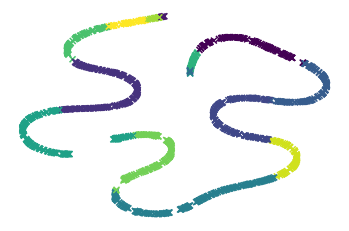
\includegraphics[width=\linewidth]{imgs/birch_lsa.png}
  \caption{LSA}
  \label{fig:birch_lsa}
\end{subfigure}%
\begin{subfigure}{.3\textwidth}
  \centering
  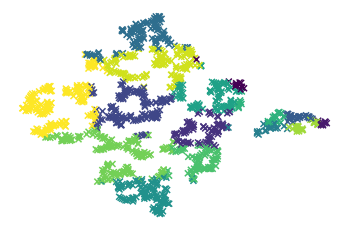
\includegraphics[width=\linewidth]{imgs/birch_spectral.png}
  \caption{Spectral Embedding}
  \label{fig:birch_spectral}
\end{subfigure}
\caption{two-dimensional representation of 15 clusters retrieved by BIRCH with different dimensionality reductions}
\label{fig:birch}
\end{figure}
In addition, the best results are also achieved by using two components.
When using BIRCH with a dimensionality reduction it is necessary, that the threshold $T$ needs to be decreased.
Otherwise, only one cluster is detected.
By decreasing it to $T=0.014$ it is again possible to extract clusters.

Because the cluster centroids are not known, the optimal number of clusters cannot be determined using the Elbow Method.
Instead, the Silhouette Score, Calinski-Harabasz-Score, and Davies-Bouldin-Score are used.
It turns out that, similar to K-Means, 10 to 15 clusters are ideal.

The stop word removal of words that occur in many clusters shows that the composition of the cluster changes a little here.
The decreasing Davies-Bouldin-Score implies that the separation between two clusters is slightly worsened by the removal, while the increasing Calinski-Harabasz-Score indicates that the clusters are slightly denser.
However, whether the clustering improves by the removal is difficult to say with the scores.

\subsubsection{Affinity Propagation}
\subsubcomment{Written by Jonas Reinwald}

As with most of the tested clustering methods, using some kind of dimensionality reduction significantly increases all metrics. As can be seen in table \ref{tab:scores_affinity_propagation}, scores without dimensionality reduction are very poor.
In these cases Affinity Propagation produced a lot of clusters, most of them containing very similar data. This is also evident in figure \ref{fig:affinity_propagation}, where the first plot shows no clear clusters at all. In contrast, the two subplots with LSA and Spectral Embedding show better clustering, albeit with still quite some overlap. 

\begin{table}[]
  \centering
  \begin{tabular}{c|c|c|c}
    Model &  \shortstack[c]{Silhouette \\ Score} & \shortstack[c]{Calinski-Harabasz \\ Score} &  \shortstack[c]{Davies-Bouldin \\ Score}  \\
    \hline
    \hline
    Affinity Propagation & 0.030495 & 2.134269 & 2.853512 \\
    \hline
    \shortstack[c]{Affinity Propagation with \\ LSA} & 0.193265 & 180.728882 & 1.26669 \\
    \hline
    \shortstack[c]{Affinity Propagation with \\ Spectral Embedding} & 0.188029 & 199.463342 & 1.30149 \\
    \hline
    \shortstack[c]{Affinity Propagation with \\ custom stopword removal} & 0.031234 & 2.141206 & 2.839059 \\
   \end{tabular}
  \caption{Metrics retrieved with Affinity Propagation}
  \label{tab:scores_affinity_propagation}
\end{table}

\begin{figure}
  \centering
  \begin{subfigure}{.3\textwidth}
      \centering
      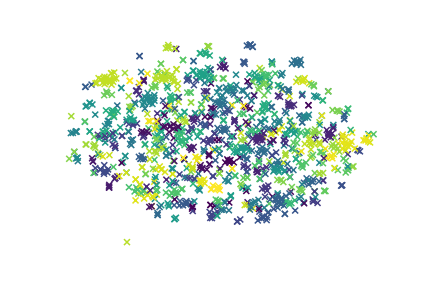
\includegraphics[width=\linewidth]{imgs/affinity_propagation.png}
      \caption{No dimensionality reduction}
      \label{fig:affinity_propagation_no_dim}
  \end{subfigure}
  \begin{subfigure}{.3\textwidth}
    \centering
    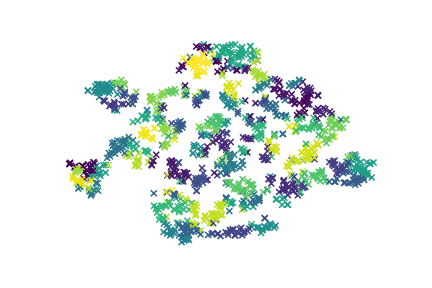
\includegraphics[width=\linewidth]{imgs/affinity_propagation_lsa.png}
    \caption{LSA}
    \label{fig:affinity_propagation_lsa}
  \end{subfigure}%
  \begin{subfigure}{.3\textwidth}
    \centering
    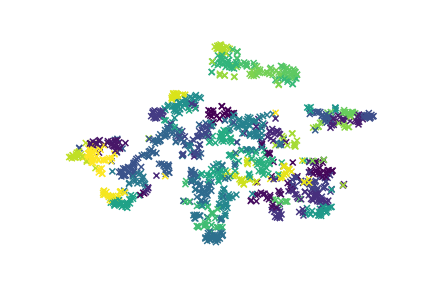
\includegraphics[width=\linewidth]{imgs/affinity_propagation_spectral.png}
    \caption{Spectral Embedding}
    \label{fig:affinity_propagation_spectral}
  \end{subfigure}
  \caption{Two-dimensional representation of clusters retrieved by Affinity Propagation with different dimensionality reduction methods}
  \label{fig:affinity_propagation}
\end{figure}

\subsubsection{Agglomerative Clustering}
\subsubcomment{Written by Jonas Reinwald}

As with Affinity Propagation, Agglomerative Clustering shows the same pattern for scores. In comparison with the former and shown in table \ref{tab:scores_agglomerative}, clustering on the raw preprocessed data produces a better Calinski-Harabasz Index, indicating slightly denser clusters, but a worse Davies-Bouldin Index, indicating less separation between clusters.
Using dimensionality reduction improves all metrics by a large margin, with LSA having one of the best scores overall. Figure \ref{fig:agglomerative} visually confirms this, with Spectral Embedding showing some perceivable distinction and LSA showing almost perfect distinction between clusters.

\begin{table}[]
  \centering
  \begin{tabular}{c|c|c|c}
    Model &  \shortstack[c]{Silhouette \\ Score} & \shortstack[c]{Calinski-Harabasz \\ Score} &  \shortstack[c]{Davies-Bouldin \\ Score}  \\
    \hline
    \hline
    Agglomerative Clustering & 0.000467 & 4.084053 & 6.231226 \\
    \hline
    \shortstack[c]{Agglomerative Clustering with \\ LSA} & 0.512373 & 10238.480445 & 0.509119 \\
    \hline
    \shortstack[c]{Agglomerative Clustering with \\ Spectral Embedding} & 0.300136 & 1029.213757 & 0.904163 \\
    \hline
    \shortstack[c]{Agglomerative Clustering with \\ custom stopword removal} & 0.001866 & 4.153627 & 6.278349 \\
   \end{tabular}
  \caption{Metrics retrieved with Agglomerative Clustering}
  \label{tab:scores_agglomerative}
\end{table}

\begin{figure}
  \centering
  \begin{subfigure}{.3\textwidth}
      \centering
      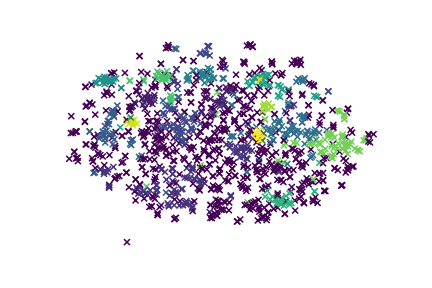
\includegraphics[width=\linewidth]{imgs/agglomerative.png}
      \caption{No dimensionality reduction}
      \label{fig:agglomerative_no_dim}
  \end{subfigure}
  \begin{subfigure}{.3\textwidth}
    \centering
    
\includegraphics[width=\linewidth]{imgs/agglomerative_lsa.png}
    \caption{LSA}
    \label{fig:agglomerative_lsa}
  \end{subfigure}%
  \begin{subfigure}{.3\textwidth}
    \centering
    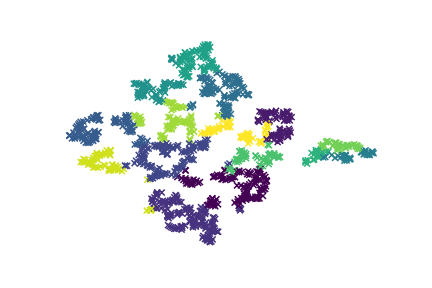
\includegraphics[width=\linewidth]{imgs/agglomerative_spectral.png}
    \caption{Spectral Embedding}
    \label{fig:agglomerative_spectral}
  \end{subfigure}
  \caption{Two-dimensional representation of clusters retrieved by Agglomerative Clustering with different dimensionality reduction methods}
  \label{fig:agglomerative}
\end{figure}

\subsubsection{DBSCAN}
\subsubcomment{Written by Jonas Reinwald}

DBSCAN did not yield any desirable results at all. As can be seen in table \ref{tab:scores_dbscan}, scores without dimensionality reduction are just as bad as with other methods and scores with dimensionality reduction are missing completely. This is because in our experiments almost all parameter settings produced only one single big cluster for normal data and one single big cluster for all tested parameter settings with LSA or Spectral Embedding, making score calculation impossible.
This is also the reason why all data points in figure \ref{fig:dbscan}, except for a few in the first subplot, are colored the same.

Because of the data-dependent threshold value (see section \ref{subsubsec:dbscan}), it might be possible to achieve better clustering by testing even more parameter values or using some kind of heuristic to find appropriate values.

\begin{table}[]
  \centering
  \begin{tabular}{c|c|c|c}
    Model &  \shortstack[c]{Silhouette \\ Score} & \shortstack[c]{Calinski-Harabasz \\ Score} &  \shortstack[c]{Davies-Bouldin \\ Score}  \\
    \hline
    \hline
    DBSCAN & -0.009707 & 2.061513 & 1.887693 \\
    \hline
    \shortstack[c]{DBSCAN with \\ custom stopword removal} & -0.010665 & 2.052975 & 1.890026 \\
   \end{tabular}
  \caption{Metrics retrieved with DBSCAN}
  \label{tab:scores_dbscan}
\end{table}

\begin{figure}
  \centering
  \begin{subfigure}{.3\textwidth}
      \centering
      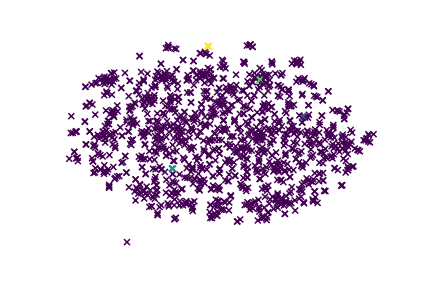
\includegraphics[width=\linewidth]{imgs/dbscan.png}
      \caption{No dimensionality reduction}
      \label{fig:dbscan_no_dim}
  \end{subfigure}
  \begin{subfigure}{.3\textwidth}
    \centering
    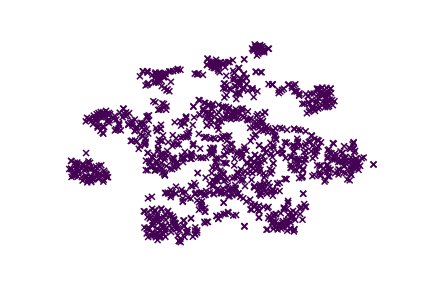
\includegraphics[width=\linewidth]{imgs/dbscan_lsa.png}
    \caption{LSA}
    \label{fig:dbscan_lsa}
  \end{subfigure}%
  \begin{subfigure}{.3\textwidth}
    \centering
    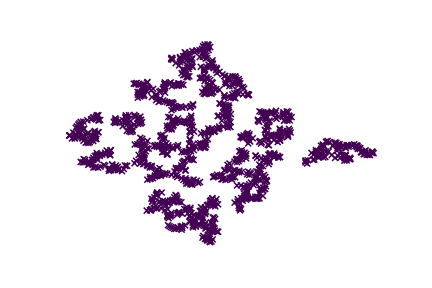
\includegraphics[width=\linewidth]{imgs/dbscan_spectral.png}
    \caption{Spectral Embedding}
    \label{fig:dbscan_spectral}
  \end{subfigure}
  \caption{Two-dimensional representation of clusters retrieved by DBSCAN with different dimensionality reduction methods}
  \label{fig:dbscan}
\end{figure}

\subsubsection{OPTICS}
\subsubcomment{Written by Jonas Reinwald}

Even though OPTICS is an improvement to the DBSCAN algorithm, results on the raw preprocessed data, as can be seen in table \ref{tab:scores_optics}, did not improve much compared to it. Depending on the parameters used OPTICS produced between 2 and 4 big clusters, with most samples belonging to the same cluster. Using dimensionality reduction only shows marginal improvements. In figure \ref{fig:optics} it is evident that more clusters are found when using dimensionality reduction, but most data points still belong to the same cluster, with LSA less so than Spectral Embedding.

\begin{table}[]
  \centering
  \begin{tabular}{c|c|c|c}
    Model &  \shortstack[c]{Silhouette \\ Score} & \shortstack[c]{Calinski-Harabasz \\ Score} &  \shortstack[c]{Davies-Bouldin \\ Score}  \\
    \hline
    \hline
    OPTICS & -0.003231 & 2.455650 & 2.620644 \\
    \hline
    \shortstack[c]{OPTICS with \\ LSA} & 0.346423 & 41.642624 & 1.53435 \\
    \hline
    \shortstack[c]{OPTICS with \\ Spectral Embedding} & -0.191176 & 13.449457 & 1.788995 \\
    \hline
    \shortstack[c]{OPTICS with \\ custom stopword removal} & -0.004380 & 2.567746 & 2.628210 \\
   \end{tabular}
  \caption{Metrics retrieved with OPTICS}
  \label{tab:scores_optics}
\end{table}

\begin{figure}
  \centering
  \begin{subfigure}{.3\textwidth}
      \centering
      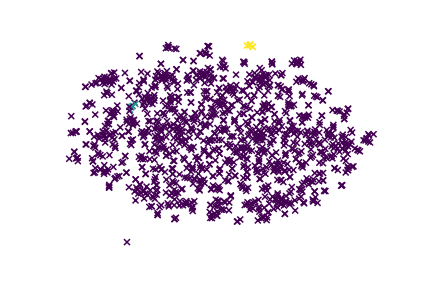
\includegraphics[width=\linewidth]{imgs/optics.png}
      \caption{No dimensionality reduction}
      \label{fig:optics_no_dim}
  \end{subfigure}
  \begin{subfigure}{.3\textwidth}
    \centering
    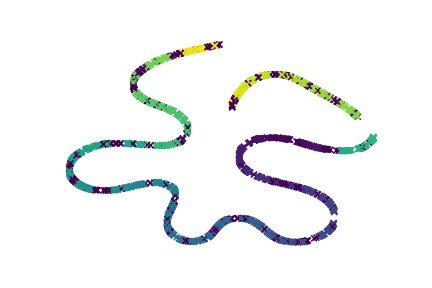
\includegraphics[width=\linewidth]{imgs/optics_lsa.png}
    \caption{LSA}
    \label{fig:optics_lsa}
  \end{subfigure}%
  \begin{subfigure}{.3\textwidth}
    \centering
    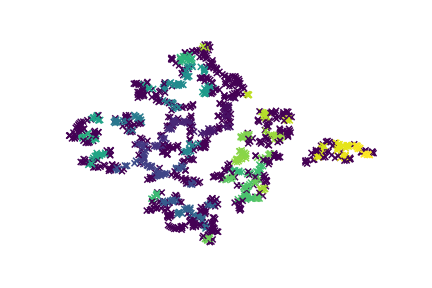
\includegraphics[width=\linewidth]{imgs/optics_spectral.png}
    \caption{Spectral Embedding}
    \label{fig:optics_spectral}
  \end{subfigure}
  \caption{Two-dimensional representation of clusters retrieved by OPTICS with different dimensionality reduction methods}
  \label{fig:optics}
\end{figure}

\subsubsection{MeanShift}
\subsubcomment{Written by Jonas Reinwald}

In contrast to DBSCAN, where experiments with dimensionality reduction resulted in only one big cluster, MeanShift does the exact opposite. Clustering with raw preprocessed data resulted in only one cluster, whereas LSA and Spectral Embedding worked better but still worse than a lot of other methods.
When looking at table \ref{tab:scores_mean_shift}, the scores for dimensionality reduction, especially LSA, are looking quite good. Unfortunately these scores do not reflect the performance of MeanShift accurately, as only two and three clusters for LSA and Spectral Embedding respectively were produced. The separation of these clusters is good, however, as can be seen in figure \ref{fig:mean_shift}.  

\begin{table}[]
  \centering
  \begin{tabular}{c|c|c|c}
    Model &  \shortstack[c]{Silhouette \\ Score} & \shortstack[c]{Calinski-Harabasz \\ Score} &  \shortstack[c]{Davies-Bouldin \\ Score}  \\
    \hline
    \hline
    \shortstack[c]{MeanShift with \\ LSA} & 0.410777 & 2443.830097 & 0.543272 \\
    \hline
    \shortstack[c]{MeanShift with \\ Spectral Embedding} & 0.474139 & 646.527661 & 0.799436 \\
   \end{tabular}
  \caption{Metrics retrieved with MeanShift}
  \label{tab:scores_mean_shift}
\end{table}

\begin{figure}
  \centering
  \begin{subfigure}{.3\textwidth}
      \centering
      
\includegraphics[width=\linewidth]{imgs/mean_shift.png}
      \caption{No dimensionality reduction}
      \label{fig:mean_shift_no_dim}
  \end{subfigure}
  \begin{subfigure}{.3\textwidth}
    \centering
    
\includegraphics[width=\linewidth]{imgs/mean_shift_lsa.png}
    \caption{LSA}
    \label{fig:mean_shift_lsa}
  \end{subfigure}%
  \begin{subfigure}{.3\textwidth}
    \centering
    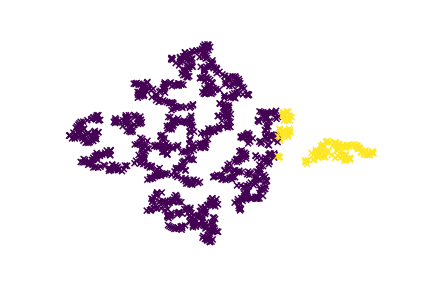
\includegraphics[width=\linewidth]{imgs/mean_shift_spectral.png}
    \caption{Spectral Embedding}
    \label{fig:mean_shift_spectral}
  \end{subfigure}
  \caption{Two-dimensional representation of clusters retrieved by MeanShift with different dimensionality reduction methods}
  \label{fig:mean_shift}
\end{figure}

\section{Conclusion}
\comment{Written by Jonas Reinwald}
In our project, we scraped a couple thousand of machine learning papers and created a dataset of unorganized text. We then created clusters with unsupervised algorithms both on the abstracts and the set of keywords.
We used the keyword clusters as ground truth for evaluation. Unfortunately, our results are not as good as we hoped they would be.

In theory, if we could achieve better results, our pipeline could be used to turn unorganized paper collections into more meaningful groups, making them organized and reducing the manual workload of researchers.
If we choose to continue work on this project, a first step towards this goal is to do a conclusive search for the best parameters of each individual algorithm.
Additionally, we have to extend our dataset to a more balanced one and create a better ground-truth from it. This would also training of learning-based clustering algorithms which might perform better than our previous approaches.
It is of course vital to then extend the approach to not only work on the subset of machine learning or computer science papers but also on a more general data set for it to be useful to a broader audience.

There are also a number of future applications this project could be used for.
We might be able to use our pipeline to propose keywords when given abstracts, by mapping generated clusters to a set of keywords and then match the given abstract to a cluster-keyword-set.
Furthermore, we think it would be possible to build and an API for accessing our results and build visualization tools and website integrations on top of that. 

\section{Note}
In the github repository state of 25.02.21 (commit: \textit{6e71af9}), there is an intermediate file \textit{data\_2021-02-01\_22-27-13.862993\_labeled.json} which has the wrong format as it was generated by an old version of our pipeline. Generating the data with the up-to-date pipeline will generate a file with the correct format. The clustering will not work with this file. It has been updated in the meantime (\url{https://github.com/DonatJR/ita_ws20/blob/main/src/data/data_2021-02-01_22-27-13.862993_labeled.json}). Please use the updated file or generate a new one.

\bibliographystyle{plain}
\bibliography{bibtex/references}

\end{document}
